\documentclass{beamer}\usepackage[]{graphicx}\usepackage[]{color}
%% maxwidth is the original width if it is less than linewidth
%% otherwise use linewidth (to make sure the graphics do not exceed the margin)
\makeatletter
\def\maxwidth{ %
  \ifdim\Gin@nat@width>\linewidth
    \linewidth
  \else
    \Gin@nat@width
  \fi
}
\makeatother

\definecolor{fgcolor}{rgb}{0.345, 0.345, 0.345}
\newcommand{\hlnum}[1]{\textcolor[rgb]{0.686,0.059,0.569}{#1}}%
\newcommand{\hlstr}[1]{\textcolor[rgb]{0.192,0.494,0.8}{#1}}%
\newcommand{\hlcom}[1]{\textcolor[rgb]{0.678,0.584,0.686}{\textit{#1}}}%
\newcommand{\hlopt}[1]{\textcolor[rgb]{0,0,0}{#1}}%
\newcommand{\hlstd}[1]{\textcolor[rgb]{0.345,0.345,0.345}{#1}}%
\newcommand{\hlkwa}[1]{\textcolor[rgb]{0.161,0.373,0.58}{\textbf{#1}}}%
\newcommand{\hlkwb}[1]{\textcolor[rgb]{0.69,0.353,0.396}{#1}}%
\newcommand{\hlkwc}[1]{\textcolor[rgb]{0.333,0.667,0.333}{#1}}%
\newcommand{\hlkwd}[1]{\textcolor[rgb]{0.737,0.353,0.396}{\textbf{#1}}}%

\usepackage{framed}
\makeatletter
\newenvironment{kframe}{%
 \def\at@end@of@kframe{}%
 \ifinner\ifhmode%
  \def\at@end@of@kframe{\end{minipage}}%
  \begin{minipage}{\columnwidth}%
 \fi\fi%
 \def\FrameCommand##1{\hskip\@totalleftmargin \hskip-\fboxsep
 \colorbox{shadecolor}{##1}\hskip-\fboxsep
     % There is no \\@totalrightmargin, so:
     \hskip-\linewidth \hskip-\@totalleftmargin \hskip\columnwidth}%
 \MakeFramed {\advance\hsize-\width
   \@totalleftmargin\z@ \linewidth\hsize
   \@setminipage}}%
 {\par\unskip\endMakeFramed%
 \at@end@of@kframe}
\makeatother

\definecolor{shadecolor}{rgb}{.97, .97, .97}
\definecolor{messagecolor}{rgb}{0, 0, 0}
\definecolor{warningcolor}{rgb}{1, 0, 1}
\definecolor{errorcolor}{rgb}{1, 0, 0}
\newenvironment{knitrout}{}{} % an empty environment to be redefined in TeX

\usepackage{alltt}
\usepackage[utf8]{inputenc}



\usepackage{url}
\ifx\hypersetup\undefined
  \AtBeginDocument{%
    \hypersetup{unicode=true,pdfusetitle,
 bookmarks=true,bookmarksnumbered=false,bookmarksopen=false,
 breaklinks=false,pdfborder={0 0 0},backref=false,colorlinks=false}
  }
\else
  \hypersetup{unicode=true,pdfusetitle,
 bookmarks=true,bookmarksnumbered=false,bookmarksopen=false,
 breaklinks=false,pdfborder={0 0 0},backref=false,colorlinks=false}
\fi

% Beamer style
%\usetheme[secheader]{Madrid}
\usetheme{CambridgeUS}
\usecolortheme[rgb={0.65,0.15,0.25}]{structure}
%\usefonttheme[onlymath]{serif}
\beamertemplatenavigationsymbolsempty


% Packages
\usepackage{dsfont, stmaryrd}
\usepackage{amsmath, amsfonts, amssymb}
\usepackage{rotating}
\usepackage{epsfig}
\usepackage{astats}
%\usepackage[all]{xy}
\usepackage{graphicx}
\usepackage{algorithm2e}

% Commands
\definecolor{darkgreen}{cmyk}{0.5, 0, 0.5, 0.5}
\definecolor{greenB}{rgb}{0.3, 0.87, 0.}
\definecolor{darkred}{rgb}{0.65,0.15,0.25}
\definecolor{darkblue}{rgb}{0.08,0.11,0.81}
%\definecolor{orange}{rgb}{0.60,0.2,0.2}
\newcommand{\blue}[1]{\textcolor{blue}{#1}}
\newcommand{\emphase}[1]{\textcolor{darkred}{#1}}
\newcommand{\emphaseBis}[1]{\textcolor{darkblue}{#1}}
\newcommand{\paragraph}[1]{\emphase{#1}}
\newcommand{\refer}[1]{\textcolor{blue}{\sl \cite{#1}}}
\newcommand{\Refer}[1]{\textcolor{blue}{\sl #1}}


%thm prop and co
\newtheorem{prop}{Proposition}

% Symbols
\def\d{\text{ d}} % Element differentiel
\newcommand{\Abf}{{\bf A}}
\newcommand{\Beta}{\text{B}}
\newcommand{\betabf}{\mbox{\mathversion{bold}{$\beta$}}}
\newcommand{\Bcal}{\mathcal{B}}
\newcommand{\BIC}{\text{BIC}}
\newcommand{\dd}{\text{d}}
\newcommand{\Cbf}{{\bf C}}
\newcommand{\dbf}{{\bf d}}
\newcommand{\Dcal}{\mathcal{D}}
\newcommand{\Esp}{\mathbb{E}}
\renewcommand{\P}{\mathbb{P}}
\newcommand{\Ebf}{{\bf E}}
\newcommand{\Ecal}{\mathcal{E}}
\newcommand{\Gcal}{\mathcal{G}}
\newcommand{\Gam}{\mathcal{G}\mbox{am}}
\newcommand{\Ibb}{\mathbb{I}}
\newcommand{\Ibf}{{\bf I}}
\newcommand{\ICL}{\text{ICL}}
\newcommand{\Cov}{\mathbb{C}\text{ov}}
\newcommand{\Corr}{\mathbb{C}\text{orr}}
\newcommand{\Var}{\mathbb{V}}
\newcommand{\Vsf}{\mathsf{V}}
\newcommand{\pen}{\text{pen}}
\newcommand{\Fcal}{\mathcal{F}}
\newcommand{\Hbf}{{\bf H}}
\newcommand{\Hcal}{\mathcal{H}}
\newcommand{\Jcal}{\mathcal{J}}
\newcommand{\Kbf}{{\bf K}}
\newcommand{\Lcal}{\mathcal{L}}
\newcommand{\Mcal}{\mathcal{M}}
\newcommand{\mbf}{{\bf m}}
\newcommand{\mum}{\mu(\mbf)}
\newcommand{\Ncal}{\mathcal{N}}
\newcommand{\Nbf}{{\bf N}}
\newcommand{\Nm}{N(\mbf)}
\newcommand{\Ocal}{\mathcal{O}}
\newcommand{\Obf}{{\bf 0}}
\newcommand{\Omegas}{\underset{s}{\Omega}}
\newcommand{\Pbf}{{\bf P}}
\newcommand{\Pcal}{\mathcal{P}}
\newcommand{\Qcal}{\mathcal{Q}}
\newcommand{\Rbb}{\mathbb{R}}
\newcommand{\Rbf}{{\bf R}}
\newcommand{\Rcal}{\mathcal{R}}
\newcommand{\sbf}{{\bf s}}
\newcommand{\Sbf}{{\bf S}}
\newcommand{\Scal}{\mathcal{S}}
\newcommand{\Ucal}{\mathcal{U}}
\newcommand{\Vcal}{\mathcal{V}}
\newcommand{\Tbf}{{\bf T}}
\newcommand{\ubf}{{\bf u}}
\newcommand{\Ubf}{{\bf U}}
\newcommand{\Wbf}{{\bf W}}
\newcommand{\xbf}{{\bf x}}
\newcommand{\Xbf}{{\bf X}}  
\newcommand{\Ybf}{{\bf Y}}
\newcommand{\Zbf}{{\bf Z}}
\newcommand{\pibf}{\mbox{\mathversion{bold}{$\pi$}}}
\newcommand{\Pibf}{\mbox{\mathversion{bold}{$\Pi$}}}
\newcommand{\Sigmabf}{\mbox{\mathversion{bold}{$\Sigma$}}}
\newcommand{\gammabf}{\mbox{\mathversion{bold}{$\gamma$}}}
\newcommand{\mubf}{\mbox{\mathversion{bold}{$\mu$}}}
\newcommand{\nubf}{\mbox{\mathversion{bold}{$\nu$}}}
\newcommand{\Thetabf}{\mbox{\boldsymbol{\Theta}}}
\newcommand{\thetabf}{\mbox{\mathversion{bold}{$\theta$}}}
\newcommand{\BP}{\text{BP}}
\newcommand{\EM}{\text{EM}}
\newcommand{\VEM}{\text{VEM}}
\newcommand{\VBEM}{\text{VB}}
\newcommand{\cst}{\text{cst}}
\newcommand{\obs}{\text{obs}}
\newcommand{\ra}{\emphase{\mathversion{bold}{$\rightarrow$}~}}
\newcommand{\QZ}{Q_{\Zbf}}
\newcommand{\Qt}{Q_{\thetabf}}
\def\argmax{\mathop{\mathrm{argmax}}}


% Directory
\newcommand{\FigSim}{}
%{/RECHERCHE/RUPTURES/MinRegionCont/Res}
\graphicspath{{figure/}{..//figure/}}
%--------------------------------------------------------------------

\title{Identifying patterns in trajectories}

\author[MP Etienne]{Marie-Pierre Etienne }

 \institute[AgroParisTech / INRA]{  AgroParisTech / INRA \\
   \bigskip
   \begin{tabular}{cccc}
    
\includegraphics[ height=1cm]{logagrotech_ABL_RVB}& 
    \hspace{.5cm} &
     \includegraphics[height=1cm]{logotype-INRA-RVB} & 
   \end{tabular} \\ 
   \bigskip
   }

\date[Movement Ecology]{Movement Ecology Workshop 2015 - Port Elizabeth}

%--------------------------------------------------------------------

%--------------------------------------------------------------------
%--------------------------------------------------------------------
\IfFileExists{upquote.sty}{\usepackage{upquote}}{}
\begin{document}



%--------------------------------------------------------------------
%--------------------------------------------------------------------

%--------------------------------------------------------------------
 \frame{\titlepage
   }
% %--------------------------------------------------------------------
% %--------------------------------------------------------------------
\frame{
\tableofcontents[subsectionstyle=hide]  }


% %--------------------------------------------------------------------
% %--------------------------------------------------------------------
\section{Introduction and Notations}


\subsection{Motivation}
\begin{frame}[fragile]{Detection of homogenous region in trajectories}

  \paragraph{Why ?}
\begin{columns}
\begin{column}{0.4\textwidth}
\begin{itemize}
\item Different behaviour
\item Link with different activities
\item Link with different environmental condition
\end{itemize}

\end{column}
\begin{column}{0.6\textwidth}



  
  \only<1>{\includegraphics[scale=0.4]{pathPractical2-1.pdf}}
\only<2>{\includegraphics[scale=0.4]{pathPractical3-1.pdf}}
\end{column}
\end{columns}
\end{frame}



\subsection{Trajectories, a certain aspect of the movement}
\begin{frame}[fragile]{Effect of sampling step}

  \only<1>{\includegraphics[scale=0.4]{pathPractical4-1.pdf}}
\only<2>{\includegraphics[scale=0.4]{pathPractical4-3.pdf}}
\only<3>{\includegraphics[scale=0.4]{pathPractical4-6.pdf}}
\only<4>{\includegraphics[scale=0.4]{pathPractical4-10.pdf}}
\only<5>{\includegraphics[scale=0.4]{pathPractical4-15.pdf}}

  \only<6>{\includegraphics[scale=0.4]{pathPractical5-1.pdf}} 
\end{frame}


\begin{frame}{Summarising trajectories}
$(t_1, \ldots, t_N)$ denotes the time acquisition and $( (x_1,y_1),  \ldots, (x_N,y_N))$ the position at those times.

\only<1>{
  \paragraph{Trajetories as Turning angle and Speed}
  \begin{columns}
  \begin{column}{0.4\textwidth}
  
  $$\boldsymbol{\Phi}=(\phi_{2}, \ldots,\phi_{N})$$
    $$\boldsymbol{S}=(S_{2}, \ldots,\S_{N}),$$
    with $S_i=dist_i/(t_i-t_{i-1})$
    \end{column}
  \begin{column}{0.6\textwidth}
  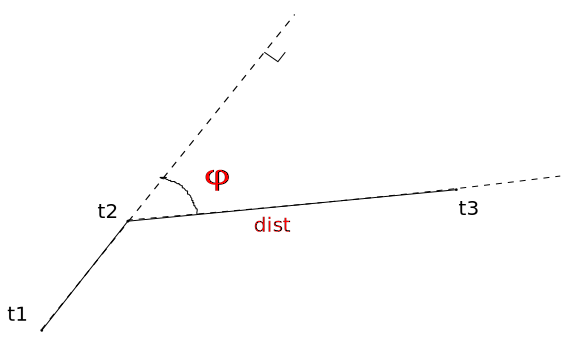
\includegraphics[scale=0.3]{Speed1.pdf}
  \end{column}
  \end{columns}
  $$ $$
}
\only<2>{
  \paragraph{Trajetories as Persistent and Normal Velocity}
  \begin{columns}
  \begin{column}{0.4\textwidth}
  
  $$\boldsymbol{V}^P=(V^P_{2}, \ldots,V^P_{N})$$
    $$\boldsymbol{V}^N=(V^N_{2}, \ldots,V^N_{N})$$
    with 
  \begin{align*}
  V^P_i&=S_i \, cos(\phi_i)\\
  V^N_i&=S_i \, sin(\phi_i)
  \end{align*}
  \end{column}
  \begin{column}{0.6\textwidth}
  \includegraphics[scale=0.3]{Speed2.pdf}
  \end{column}
  \end{columns}
}
\end{frame}


\begin{frame}{Trajectories data}
\paragraph{How trajectories data migh be considered?}
\begin{itemize}
\item A sequence of (time, position)
\item Turning angle and speed sequences
\item Persistent and Normal Velocity sequences
\end{itemize}
\pause
\paragraph{What is affected by sampling?}
\begin{itemize}
\item A sequence of (time, position)
\item Turning angle and speed sequences
\item Persistent and Normal Velocity sequences
\end{itemize}
\pause
\paragraph{Model approach:}
\begin{itemize}
\item Most methods don't consider the two phenomena : movement and sampling process.
  \item Results will be closely dependent of the sampling step.
  \end{itemize}
\end{frame}

\subsection*{Convention}


\begin{frame}{Convention}
\paragraph{Notation:}
{\small
\begin{itemize}
\item $\Ybf = (Y_1, \ldots, Y_n) = $ observed data (typically Speed)
 \item $\Zbf $ unobserved data (typically State, for mixture  and Hidden Markov model)
 \item \thetabf = the unknown parameters of $\Ybf$ and $\Zbf$.
\end{itemize}
}
\pause
\paragraph{Graphical Representation (DAG):}  \medskip
\begin{columns}
\begin{column}{0.3\textwidth}
\centering{Change point}\\ \smallskip
\includegraphics[scale=0.4]{Dag1.pdf}
\end{column}
\pause

\begin{column}{0.3\textwidth}
\centering{Mixture}\\ \smallskip
\includegraphics[scale=0.4]{Dag2.pdf}
\end{column}
\pause
\begin{column}{0.3\textwidth}
\centering{HMM}\\ \smallskip
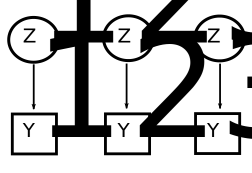
\includegraphics[scale=0.4]{Dag3.pdf}
\end{column}
\end{columns}
\end{frame}
%#show plan at the beginning of each secion except the first one
\AtBeginSection[]
{
 \begin{frame}<beamer>
 \frametitle{Plan}
 \tableofcontents[currentsection]
 \end{frame}
}

% %--------------------------------------------------------------------
% %--------------------------------------------------------------------
\section{Change point model}

\subsection{Goal and Model}
\subsection*{Goal}
  \frame{\frametitle{Change point detection context}
    \begin{tabular}{p{0.5\textwidth} p{0.4\textwidth}}
    \begin{tabular}{p{\textwidth}}
        \includegraphics<1>[height=.6\textheight]{rawSignal}
        \includegraphics<2>[height=.6\textheight]{segmentedSignal}
      \end{tabular}
    &  
      \begin{tabular}{p{0.4\textwidth}}
        \onslide<1>{ \emph{Goal : } Identifying homogenous region and abrupt changes in the signal.\\}
        \onslide<2>{ These \textcolor{red}{regions} may be interpreted afterwards.\\}
    \end{tabular}
  \end{tabular}
  }

  \frame{\frametitle{Change point detection context}

  Two possible statistical point of view : 
  \begin{itemize}
  \item Bayesian approach : the output is the posterior probability for each point to be a change point.
  \item \emph{Frequentist} approach : the output is the best segmentation (according to a given critrion)
  \end{itemize}
  }

\subsection*{Model}
\frame{\frametitle{Underlying model}
  \only<1>{ General framework~:}
  \only<2>{\textcolor{red}{Change point detection in the trend~:} }
  \begin{itemize}
  \item Data $Y_1,\ldots,Y_n$ are drawn from a given pdf, driven by unknown parameter $\theta$
    \begin{equation*}
      Y_t \sim f_{\theta}(.)  \ \ 
    \end{equation*}
  \item
    $\theta$ values change at  $K-1$ unknow instants, the change point~:
    $t_1,\ldots,t_{K-1}$ :
    \only<1>{
      \begin{equation*}
        Y_t \sim f(\theta_k) \ \ \mbox{if $t$ in region $I_k=[t_{k-1}+1,t_{k}]$}
      \end{equation*}}
    \only<2>{
      \textcolor{red}{
        \begin{equation*}
          Y_t=\mu_k + E_t \quad \{E_t\} \mbox{i.i.d.} \sim \Ncal(0,\sigma^2) \mbox{ if $t$ in portion $I_k$,}
        \end{equation*}
        for  $k=1,\ldots,K$.
      } }
 \par
 \medskip
\noindent Remark : $K-1$ change points  $\Leftrightarrow$ $K$ regions.
\end{itemize}
 } 

 
 \subsection*{Estimation}
 \frame{\frametitle{Estimation procedure}
   \begin{itemize}
   \item Unknown parameters : $\mu_1, \ldots, \mu_K$, $\sigma$, and $T_1, \ldots, T_K$,\\
     but  also \textcolor{red}{K} itself.
\pause
   \item Estimation Procedure
     \begin{itemize}
       \item for a given $K$,  $\mu_1, \ldots, \mu_K$, $\sigma_1, \ldots,\sigma_K$, and $T_1, \ldots, T_K$ are estimated using maximum likelihood (and dynanic programming)
       \item K is chosen using penalized likelihood approach
       \end{itemize}
     \end{itemize} 
         \pause
         \begin{tabular}{p{0.4\textwidth} p{0.4\textwidth}}
           \begin{tabular}{p{0.4\textwidth}}
             Likelihood increases with the number of segment, but
           \end{tabular}
           &  \pause
           \begin{tabular}{p{0.4\textwidth}}
             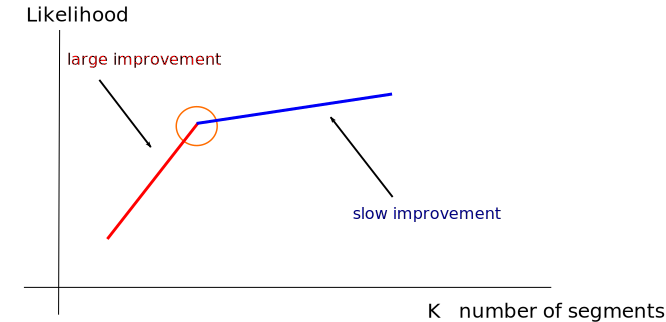
\includegraphics[scale=0.3]{LikelihoodProfile}
           \end{tabular}
         \end{tabular}
   }


\frame{\frametitle{Estimation procedure}

\paragraph{Likelihood}
{\small
\begin{eqnarray*}
2 log(P_K (T, \theta)) & = & 2 \sum_{k=1}^K \log f(\{Y_t\}_{t \in
I_k};
\theta_k) = 2 \sum_{k=1}^K \sum_{t \in I_k}\log f(Y_t; \theta_k) \\
& = & -n \log \sigma^2 - \frac1{\sigma^2} \sum_{k=1}^K \sum_{t \in
  I_k} (Y_t - \mu_k)^2 + \mbox{cst}.
\end{eqnarray*}
}

\paragraph{Estimations}
\begin{equation*}
 (\hat{T},\hat{\theta})=
  \argmax_{(T,\theta)} log(P_K (T, \theta))
\end{equation*}

\paragraph{If the change points are known}
\begin{columns}
\begin{column}{0.5\textwidth}
\begin{equation*}
\widehat{\mu}_k = \frac1{n_k} \sum_{t \in I_k} Y_t
\end{equation*}
\end{column}
\begin{column}{0.5\textwidth}
  $$
  \widehat{\sigma}^2 =  \frac1{n} \sum_{k=1}^K \sum_{t \in I_k} (Y_t -  \widehat{\mu}_k)^2
  $$
\end{column}
\end{columns}
}

\begin{frame}[fragile]{Finding the K-1 change points}
\only<1-3>{
\paragraph{Considering all possible segmentations, } the best segmentation minimizes 
$$
J_k(1, n) = \sum_{k=1}^K \sum_{t \in I_k} (Y_t - \widehat{\mu}_k)^2.
$$
\pause
\paragraph{But, } $$\left( \begin{array}{c} n-1 \\ K-1 \end{array}\right)$$ possible choices for the $K-1$ positions
:\\
  \centerline{$\Rightarrow$ Practically impossible even for small $K$ and $n$}
  \medskip 
  \pause
  
  $K=10$, $n=200$,  $\left( \begin{array}{c} K-1 \\ n-1 \end{array}\right)\approx 2. 10^{16}$
}

\paragraph{Dynamic programming,} with complexity ($\mathcal{O}(n^2)$).


%possible only because the quantity of interest is the sum over all segments 

%%%%%%%%%%%%%%%%%%%%%%%%%%%%%%%%%%%%%%%%%%%%%%%%%%%%%%%%%%%%%%%%%%%%%%
%%%%%%%%%%%%%%%%%%%%%%%%%%%%%%%%%%%%%%%%%%%%%%%%%%%%%%%%%%%%%%%%%%%%%%
\only<4>{\centerline{\sl Sub-paths of the optimal path are themselves
optimal,} 
Bellmann optimality 

\vspace{3.8cm}
$$ $$ }
\only<5>{
\begin{description}

\item[Initialisation:] Compute for $0 \leq i < j \leq n$, cost of portion $I_{ij}$~:
 $$
 J_1(i, j) = \sum_{t=i+1}^j (Y_t - \widehat{\mu})^2
 $$
\item[Etape $k$:] Compute for $2 \leq k \leq K$, $J_k(i, j)$ the cost of the best segmentation in $k$ segments between $i$ and $j$.
  $$
  J_k(i, j) = \min_{i < h <j} \left[J_{k-1}(i, h) + J_1(h+1,  j)\right].
  $$
\end{description}
}
\end{frame}


\subsection{Example}
\subsection*{ Toy Example}
   \begin{frame}[fragile]{How to perform this segmentation approach ?}

 
\begin{columns}
\begin{column}{0.4\textwidth}
\begin{knitrout}\tiny
\definecolor{shadecolor}{rgb}{0.969, 0.969, 0.969}\color{fgcolor}\begin{kframe}
\begin{alltt}
\hlkwd{load}\hlstd{(}\hlstr{"../Data/dataSegmentation.Rd"}\hlstd{)}
\hlkwd{summary}\hlstd{(Profil.seg)}
\end{alltt}
\begin{verbatim}
   Min. 1st Qu. 
 0.8904  4.8720 
 Median    Mean 
 5.6990  5.3660 
3rd Qu.    Max. 
 6.3070  8.9400 
\end{verbatim}
\begin{alltt}
\hlkwd{plot}\hlstd{(Profil.seg)}
\end{alltt}
\end{kframe}
\end{knitrout}
\end{column}
\begin{column}{0.5\textwidth}
\includegraphics[scale=0.35]{segCode2-1.pdf}
\end{column}
\end{columns}
\end{frame}

\subsection*{Practical Example}
   \begin{frame}[fragile]{How to perform this segmentation approach ?}
\begin{columns}
\begin{column}{0.4\textwidth}
\begin{knitrout}\tiny
\definecolor{shadecolor}{rgb}{0.969, 0.969, 0.969}\color{fgcolor}\begin{kframe}
\begin{alltt}
\hlkwd{library}\hlstd{(}\hlstr{'cghseg'}\hlstd{)}
\hlcom{## format data into CGHdata}
\hlstd{signalCGH}    \hlkwb{<-} \hlkwd{new}\hlstd{(}\hlstr{"CGHdata"}\hlstd{,}\hlkwc{Y}\hlstd{=Profil.seg)}
\hlstd{CGHo}         \hlkwb{<-} \hlkwd{new}\hlstd{(}\hlstr{"CGHoptions"}\hlstd{)}
\hlkwd{calling}\hlstd{(CGHo)}\hlkwb{<-} \hlnum{FALSE} \hlcom{## no classification }
\hlstd{segSignal}   \hlkwb{<-} \hlkwd{uniseg}\hlstd{(}\hlkwc{.Object}\hlstd{=signalCGH,}\hlkwc{CGHo}\hlstd{=CGHo)}
\hlstd{segSignalProf} \hlkwb{<-} \hlkwd{getsegprofiles}\hlstd{(segSignal)}
\hlkwd{plot}\hlstd{(Profil.seg)}
\hlkwd{lines}\hlstd{(}\hlnum{1}\hlopt{:}\hlkwd{length}\hlstd{(segSignalProf),}
      \hlstd{segSignalProf,} \hlkwc{type}\hlstd{=}\hlstr{"s"}\hlstd{,} \hlkwc{col}\hlstd{=}\hlnum{2}\hlstd{,} \hlkwc{lwd}\hlstd{=}\hlnum{2}\hlstd{)}
\end{alltt}
\end{kframe}
\end{knitrout}
\end{column}
\begin{column}{0.5\textwidth}
\includegraphics[scale=0.35]{segCode3-1.pdf}
\end{column}
\end{columns}
\end{frame}
% 

 
 \begin{frame}[fragile]{Do it yourself}

\begin{columns}
\begin{column}{0.4\textwidth}
\begin{knitrout}\tiny
\definecolor{shadecolor}{rgb}{0.969, 0.969, 0.969}\color{fgcolor}\begin{kframe}
\begin{alltt}
\hlkwd{load}\hlstd{(}\hlkwc{file}\hlstd{=}\hlstr{"../Data/trajEx.Rd"}\hlstd{)}
\hlkwd{plot}\hlstd{(traj.ex,} \hlkwc{addpoints} \hlstd{= F)}
\hlkwd{legend}\hlstd{(}\hlstr{"bottomleft"}\hlstd{,}\hlkwc{pch}\hlstd{=}\hlkwd{c}\hlstd{(}\hlnum{2}\hlstd{,} \hlnum{0}\hlstd{),} \hlkwc{col}\hlstd{=}\hlkwd{c}\hlstd{(}\hlnum{4}\hlstd{,}\hlnum{2}\hlstd{),}
       \hlkwc{legend}\hlstd{=}\hlkwd{c}\hlstd{(}\hlstr{"Start"}\hlstd{,} \hlstr{"End"}\hlstd{),} \hlkwc{bty} \hlstd{=} \hlstr{"n"}\hlstd{,}
       \hlkwc{pt.lwd} \hlstd{=} \hlkwd{c}\hlstd{(}\hlnum{1.5}\hlstd{,}\hlnum{1.5}\hlstd{),} \hlkwc{pt.cex} \hlstd{=} \hlkwd{c}\hlstd{(}\hlnum{1.5}\hlstd{,}\hlnum{1.5}\hlstd{))}
\end{alltt}
\end{kframe}
\end{knitrout}
\end{column}
\begin{column}{0.5\textwidth}
\includegraphics[scale=0.35]{Practical1-1.pdf}
\end{column}
\end{columns}
\end{frame}

\subsection{ClusteringSegmentation}
%%%%%%%%%%%%%%%%%%%%%%%%%%%%%%%%%%%%%%%%%%%%%%%%%%%%%%%%%%
\begin{frame}{When Segmentation is not sufficient}
$$
\begin{tabular}{cc}
  Pure segmentation & Segmentation + classification \\
  \includegraphics[scale=0.3]{FigSegClas-1.pdf} &
  \includegraphics[scale=0.3]{FigSegClas-2.pdf} 
  \end{tabular}
$$
\end{frame}
\begin{frame}{Segmentation-Clustering}
 \begin{itemize}
 \item Assuming a \textcolor{blue}{secondary underlying
     structure} of the segments into $P$ groups with weights
   $\pi_1,...,\pi_P (\sum_p \pi_p=1)$.
 \item Let's define \emphase{hidden variables $Z_{kp}$}, indicators of the
   \emphase{group to which segment $k$ belongs}.
 \item $\pi_p$ denotes the \emphase{proportion} of group $p$.
 \item The \emphase{distribution of the signal} given the group of the
     segment is
  \begin{align*}
   t \in I_k, k \in p &\qquad \Rightarrow \qquad Y_t \sim
   \Ncal(m_{\emphase{p}}, \sigma^2)\\
   Y^k|Z_{kp}=1 &\sim \Ncal( m_p, \sigma^2 ).
   \end{align*}
 %\item It is a model of \textblue{segmentation/clustering}.
 \item The \emphase{parameters of this model} are
   \begin{eqnarray*}
   \mbox{the breakpoint positions:} \quad T&=&(t_1, ..., t_{K-1}),\\
     \mbox{the mixture characteristics:} \quad \Theta&=&(\pi_1,\hdots,\pi_P;\mu_1,\hdots,\mu_P,\sigma).
   \end{eqnarray*}
\end{itemize}
\end{frame} 


\begin{frame}{Hybrid algorithm}
\only<1>{
\paragraph{2 levels of statistical units} 
 \begin{itemize}
 \item  The inference of the \emphase{breakpoints $T$}
   is made at the \emphase{position level $t$};
 \item  The inference of the \emphase{groups (status)
     ($\Theta, \tau_{kp}$)} is made at the \emphase{segment level $k$}.
 \end{itemize}
} 
\only<2>{
 \paragraph{Alternate parameters estimation with $K$ and $P$ known}
 \begin{enumerate}
 \item  When $T$ is fixed, the
   \textcolor{blue}{Expectation-Maximisation (EM)} algorithm estimates
   $\Theta$;
   $$
   \hat{\Theta}^{(h+1)}=\underset{\Theta}{\arg\max} \left\{\log
     \Lcal_{KP}\left(\Theta,T^{(h)}\right) \right\}. 
  $$
   $$
   \log \Lcal_{KP}( \hat{\Theta}^{(h+1)}; \hat{T}^{(h)})
   \geq \log \Lcal_{KP}(\hat{\Theta}^{(h)};
  \hat{T}^{(h)})
  $$
 \item  When $\Theta$ is fixed, \textcolor{blue}{dynamic
     programming} estimates $T$;
    $$
   \hat{T}^{(h+1)}=\underset{T}{\arg\max} \left\{\log
     \Lcal_{KP}\left(\hat{\Theta}^{(h+1)},T\right) \right\}. 
  $$
   $$
   \log \Lcal_{KP}(\hat{\Theta}^{(h+1)}; \hat{T}^{(h+1)})
   \geq \log \Lcal_{KP}(\hat{\Theta}^{(h+1)};
   \hat{T}^{(h)})
   $$
   \end{enumerate} 
}
\end{frame}
 

\subsection{Example}
\subsection*{Toy Example}
   \begin{frame}[fragile]{How to perform this segmentation/clustering approach ?}
 
\begin{columns}
\begin{column}{0.4\textwidth}
\begin{knitrout}\tiny
\definecolor{shadecolor}{rgb}{0.969, 0.969, 0.969}\color{fgcolor}\begin{kframe}
\begin{alltt}
\hlcom{## format data into CGHdata}
\hlkwd{calling}\hlstd{(CGHo)}\hlkwb{<-} \hlnum{TRUE} \hlcom{## no classification }
\hlstd{CGHo}\hlopt{@}\hlkwc{nblevels}\hlkwb{=}\hlnum{2}
\hlstd{segSignal}   \hlkwb{<-} \hlkwd{uniseg}\hlstd{(}\hlkwc{.Object}\hlstd{=signalCGH,}\hlkwc{CGHo}\hlstd{=CGHo)}
\hlstd{segSignalProf} \hlkwb{<-} \hlkwd{getsegprofiles}\hlstd{(segSignal)}
\hlkwd{plot}\hlstd{(Profil.seg)}
\hlkwd{lines}\hlstd{(}\hlnum{1}\hlopt{:}\hlkwd{length}\hlstd{(segSignalProf),}
      \hlstd{segSignalProf,} \hlkwc{type}\hlstd{=}\hlstr{"s"}\hlstd{,} \hlkwc{col}\hlstd{=}\hlnum{2}\hlstd{,} \hlkwc{lwd}\hlstd{=}\hlnum{2}\hlstd{)}
\end{alltt}
\end{kframe}
\end{knitrout}
\end{column}
\begin{column}{0.5\textwidth}
\includegraphics[scale=0.35]{segCode4-1.pdf}
\end{column}
\end{columns}
\end{frame}

\subsection*{Practical Example}
\begin{frame}[fragile]{Do it yourself}
\end{frame}
% %--------------------------------------------------------------------
% %--------------------------------------------------------------------
\section{Mixture Model}

\subsection{Model}

\begin{frame}[fragile]{Problem presentation}

\begin{columns}
\begin{column}{0.5\textwidth}
\only<2>{\includegraphics[scale=0.3]{mixCode1-5.pdf}}
\only<3->{\paragraph{Basic idea :}\\
 "Expert" threshold $s$ \\  
 $$ State_i=1 \quad \mbox{if} Y_i<s$$
 $$ State_i=2 \quad \mbox{if} Y_i\geq  s $$
}
\only<5->{\paragraph{Improvement:}\\
 \textcolor{blue}{Estimating} the threshold s and  reconstruction of the hidden state (colour)\\
 Compute the \textcolor{blue}{probability to belong} to State 1 or 2.\\
}
 \only<6->{
 \bigskip
   \centering{$\Longrightarrow$ \textcolor{red}{Mixture Model}}
 }
 \end{column}
 \begin{column}{0.4\textwidth}

 \only<1>{\includegraphics[scale=0.3]{mixCode1-1.pdf}}
 \only<2>{\includegraphics[scale=0.3]{mixCode1-2.pdf}}
 \only<3>{\includegraphics[scale=0.3]{mixCode1-3.pdf}}
 \only<4->{\includegraphics[scale=0.3]{mixCode1-4.pdf}}
\end{column}
\end{columns}
\end{frame}

%%-----------------------------------------------------------------%%
%%-----------------------------------------------------------------%%

\begin{frame}[fragile]{Proposed model}
\paragraph{Model}
For a given number of states $K$, 
\begin{itemize}
\item
 \blue{Modelling $Z$}: $\pi_k=\P(Z_i=k), \quad k=1,\ldots, K, \quad \sum_k \pi_k=1$\par
 $Z_i \overset{i.i.d}{\sim} \Mcal(1, \pibf), \quad P(Z_{ik}=1)=\pi_k$
 \item \blue{Modelling $Y$}: The $Y_i's$ are assumed to be independent  conditionnaly to $\Zbf$ : $(Y_i\vert Z_i = k) \overset{i.i.d}{\sim} f_{\theta_k}().$
\end{itemize}
 \onslide<2->{\centering{\blue{Model parameters are $\pibf$ and $\thetabf$}}\par}
 \onslide<3->{\centering{\includegraphics[scale=0.4]{Dag2.pdf}}}
\end{frame}

\begin{frame}[fragile]{Proposed model}
\paragraph{Model}
For a given number of states $K$, 
\begin{itemize}
\item
 \blue{Modelling $Z$}: $\pi_k=\P(Z_i=k), \quad k=1,\ldots, K, \quad \sum_k \pi_k=1$\par
 $Z_i \overset{i.i.d}{\sim} \Mcal(1, \pibf)$
 \item \blue{Modelling $Y$}: The $Y_i's$ are assumed to be independent  conditionnaly to $\Zbf$ : $(Y_i\vert Z_i = k) \overset{i.i.d}{\sim} f_{\theta_k}().$
\end{itemize}
\begin{columns}
  \begin{column}{0.45\textwidth}
\begin{knitrout}\tiny
\definecolor{shadecolor}{rgb}{0.969, 0.969, 0.969}\color{fgcolor}\begin{kframe}
\begin{alltt}
\hlstd{K} \hlkwb{<-} \hlnum{2}\hlstd{; N} \hlkwb{<-} \hlnum{400}\hlstd{; mu} \hlkwb{<-} \hlkwd{c}\hlstd{(}\hlnum{3}\hlstd{,} \hlnum{7}\hlstd{); sigma} \hlkwb{<-} \hlkwd{c}\hlstd{(}\hlnum{1}\hlstd{,}\hlnum{1.5}\hlstd{)}
\hlstd{Z} \hlkwb{<-} \hlkwd{sample}\hlstd{(}\hlnum{1}\hlopt{:}\hlnum{2}\hlstd{,} \hlkwc{size} \hlstd{= N,} \hlkwc{replace}\hlstd{=T,} \hlkwc{prob}\hlstd{=}\hlkwd{c}\hlstd{(}\hlnum{0.3}\hlstd{,} \hlnum{0.7}\hlstd{))}
\hlkwd{plot}\hlstd{(Z,} \hlkwc{col}\hlstd{=Z}\hlopt{+}\hlnum{1}\hlstd{,} \hlkwc{pch}\hlstd{=}\hlnum{15}\hlstd{)}
\hlstd{Y.mixture} \hlkwb{<-} \hlkwd{rnorm}\hlstd{(N,} \hlkwc{mean}\hlstd{=mu[Z],} \hlkwc{sd}\hlstd{=sigma[Z])}
\hlkwd{plot}\hlstd{(Y.mixture,} \hlkwc{col}\hlstd{=Z}\hlopt{+}\hlnum{1}\hlstd{,} \hlkwc{pch}\hlstd{=}\hlnum{19}\hlstd{)}
\end{alltt}
\end{kframe}
\end{knitrout}
 \end{column}
  \begin{column}{0.45\textwidth}
    \only<3>{\includegraphics[height=3cm, width=6cm]{mixCode2-1.pdf}}
    \only<4->{\includegraphics[scale=0.25]{mixCode2-2.pdf}}
  \end{column}
  \end{columns}
\end{frame}

\begin{frame}[fragile]{Model Properties}
\begin{itemize}
\item Couples $\{(Y_i, Z_i)\}$ are i.i.d.
\item \blue{Label switching}:\\ the model is invariant for any permutation of the labels $\{1,
  \dots, K\}$ $\Rightarrow$ the mixture model has \emphase{$K!$
    equivalent definitions}.
\item\blue{Distribution of a $Y_i$:}\\
$$P(Y_i)=\sum_{k=1}^K P(Y_i, Z_i=k)=\textcolor{blue}{P(Z_i=k)} \textcolor{magenta}{P(Y_i | Z_i=k)} $$
\item\blue{Distribution of $\Ybf$:}\\
{\small
\begin{eqnarray*}
P(\Ybf ; \thetabf, \pibf)= \prod_{i=1}^n \sum_{k=1}^K P(Y_i , Z_i=k)  
&=& \prod_{i=1}^n \sum_{k=1}^K \textcolor{blue}{P(Z_i=k)} \textcolor{magenta}{P(Y_i | Z_i=k)} \\ 
&=& \prod_{i=1}^n \sum_{k=1}^K \textcolor{blue}{\pi_k} \textcolor{magenta}{f_{\theta_k}(Y_i)} 
\end{eqnarray*}
}
\end{itemize}
\end{frame}

\subsection{Parameter estimation}
%%-----------------------------------------------------------------%%
%%-----------------------------------------------------------------%%


\begin{frame}{Statistical inference of incomplete data models} 
 \paragraph{Maximum likelihood estimate:} We are looking for
  $$
  (\widehat{\thetabf},\widehat{\pibf}) = \arg\max_{\thetabf, \pibf} \log P(\Ybf; \thetabf, \pibf)
  $$
  \begin{itemize}
  \item Likelihood of the observed data (or observed likelihood):
    $$
    \log P(\Ybf; \thetabf, \pibf)=
    \sum_{i=1}^n \log \left[\sum_{k=1}^K \pi_k f_{ \theta_k}(Y_i)\right]
    $$
  \item No analytical estimators. 
  \item  It is not always possible since this sum typically involves $K^n$ terms : $2^{100}\approx10^{30}$, the computation will take $10^{10}$ years on a 2014 computer. 
  \item Brute force algorithm is not the way
  \end{itemize}
\end{frame}
%%-----------------------------------------------------------------%%
%%-----------------------------------------------------------------%%


\begin{frame}{And what if $\Zbf$ were observed  ?}
The complete likelihood is 
\begin{align*}
    \log P(\Ybf, \Zbf; \thetabf, \pibf) &=\log P(\Zbf; \pibf) + \log P(\Ybf\vert \Zbf; \thetabf)\\
      & =  \sum_i \sum_k Z_{ik} \log \pi_k + \sum_i \sum_k Z_{ik} \log
    f_{\theta_k}(Y_i) \\
    & =  \sum_i \sum_k Z_{ik} [\log \pi_k + \log
      f_{\theta_k}(Y_i)].
\end{align*}
  
Now, the sum contains $nK$ ($200$ if $n=100$ and $K=2$) terms.  It is much easier.
\pause

\centering{\textcolor{red}{Unfortunately $\Zbf$ are unknown.} }
\pause

\bigskip

\textcolor{red}{Idea:} Replace $Z_i$, by our best guess, that is~:
$$
\tau_{ik}:=\Esp(Z_i = k | Y_i)=P(Z_i = k | Y_i)
$$  
\end{frame}

\begin{frame}{More generally - EM algorithm}
\begin{columns}
\begin{column}{0.2\textwidth}
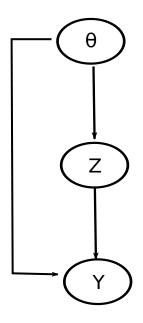
\includegraphics[scale=0.5]{ModHier.pdf}
\end{column}
\begin{column}{0.8\textwidth}
\paragraph{Bayes Formula}
{\small
\begin{align*}
P(\Ybf, \Zbf;\thetabf) & = P(\Ybf\vert \Zbf; \thetabf) P(\Zbf; \thetabf),\\
& = \textcolor{orange}{P(\Zbf\vert \Ybf; \thetabf) P(\Ybf; \thetabf).}
\end{align*}
Therefore,
\begin{align*}
\log P(\Ybf; \thetabf) & = \log \left \lbrace P(\Ybf, \Zbf;\thetabf) / P(\Zbf\vert \Ybf; \thetabf) \right\rbrace\\
& = \log P(\Ybf, \Zbf;\thetabf) - \log P(\Zbf\vert \Ybf; \thetabf) \\
\end{align*}
For a given $\thetabf_0$, we may compute $P_{\thetabf_0}=P(\Zbf\vert \thetabf_0, \Ybf)$ and
\begin{align*}
\log P(\Ybf; \thetabf) &= \Esp_{\thetabf_0}(\log P(\Ybf, \Zbf;\thetabf)) - \Esp_{\thetabf_0}(\log P(\Zbf\vert \Ybf; \thetabf))\\
  & = Q(\thetabf, \thetabf_0) - H(\thetabf, \thetabf_0)
  \end{align*}}
\end{column}
\end{columns}
\end{frame}


\begin{frame}{More generally - EM algorithm}
\begin{columns}
\begin{column}{0.2\textwidth}
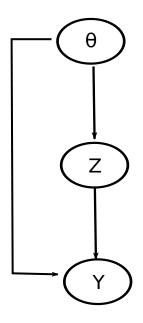
\includegraphics[scale=0.5]{ModHier.pdf}
\end{column}
\begin{column}{0.8\textwidth}
{\small
Since 
$$\log P(\Ybf; \thetabf)  = Q(\thetabf, \thetabf_0) - H(\thetabf, \thetabf_0),$$
and $H(\thetabf, \thetabf_0)$ achieves its maximum in $\thetabf_0$,
\begin{align*}
\log P(\Ybf; \thetabf)- \log P(\Ybf; \thetabf_0)  = & \textcolor{orange}{(Q(\thetabf, \thetabf_0) - Q(\thetabf, \thetabf_0))} +\cr
&\textcolor{green}{(H(\thetabf_0, \thetabf_0)-H(\thetabf, \thetabf_0))}.
\end{align*}
}

\paragraph{Expectation - Maximization algorithm}
\begin{enumerate}
\item Phase E : \\
Calculate  $Q(\thetabf,\thetabf^{k})$ for every $\thetabf$.
\item Phase M :\\ Define  
$\thetabf^{k+1}=argmax\, Q(\thetabf,\thetabf^{k})$
\end{enumerate}
\end{column}
\end{columns}
\end{frame}

\begin{frame}{EM algorithm for independent mixture model}
\begin{align*}
  Q(\thetabf,\thetabf^{(\ell)}) & = \Esp_{\thetabf^{(\ell)}}(\log P(\Ybf, \Zbf;\thetabf))\\
  &= \Esp_{\thetabf^{(\ell)}} \left\{\sum_i \sum_k Z_{ik} [\log \pi_k + \log
       f_{\theta_k^{(\ell)}}(Y_i)] \right\}\\
  &= \sum_i \sum_k \Esp_{\thetabf^{(\ell)}} (Z_i = k | Y_i) \log\left[\pi_k f_{\theta_k^{(\ell)}}(Y_i)\right]
  \end{align*}
   Recall that $\tau_{ik}^{(\ell)}:=P_{\thetabf^{(\ell)}}(Z_i = k | Y_i )$
   $$Q(\thetabf;\thetabf^{(\ell)})
     =\sum_i \sum_k \tau_{ik}^{(\ell)} \log \pi_k +  \sum_i \sum_k \tau_{ik}^{(\ell)}\log f_{\theta_k^{(\ell)}}(Y_i)$$
     $\rightarrow$ Need to estimate $\tau_{ik}^{(\ell)}$
\end{frame}

\begin{frame}{EM algorithm for independent mixture model}
    \begin{itemize}
    \item Initialisation of $\thetabf^{(0)}=(\pi_1, ..., \pi_K, \theta_1, ..., \theta_K)^{(0)}$.
  \pause
  \item Alternate  
      \begin{description}
      \item[E-step] Calculation of $\tau^{(\ell)}_{ik}=P(Z_i = k | y_i, \thetabf^{(\ell-1)}) = \frac{\pi^{(\ell-1)}_k f_{\theta^{(\ell-1)}_k}(y_i)}{\sum_{k'} \pi^{(\ell-1)}_{k'}f_{\theta^{(\ell-1)}_{k'}}(x_i)}$

      \item[M-step] Maximization of
        $$
        (\pibf, \gammabf) \longmapsto \sum_i \sum_k \tau_{ik}^{(\ell)} [\log \pi_k +
          \log f(x_i; \gamma_k)]
        $$
      \end{description} 
    \end{itemize}
\end{frame}

\begin{frame}{In our situation}
\begin{itemize}  
\item $Z \in \{1,2\}$: $P(Z=1)=\pi_1$ and $P(Z=2)=1-\pi_1$  
\item For $k=1$ or $2$, $(X|Z=k) \sim \Ncal(\mu_k, \sigma_k^2)$ 
\item the parameter vector is $(\pi, \mu_1, \mu_2, \sigma_2^2, \sigma_2^2)$
\item[] Assume that $n$ observations $y_1, y_2, ..., y_n$ are available
\item The parameter estimators  at step $(\ell+1)$ of the EM algorithm 
are given by:
\end{itemize}
\bigskip
   \begin{eqnarray*}
     \widehat{\pi}_1^{(\ell+1)} & = & \frac1{n} \sum_{i=1}^n \tau_{i1} ^{(\ell)}, \\
     \widehat{\mu}_k^{(\ell+1)} & = & \frac1{\sum_{i=1}^n  \tau_{ik} ^{(\ell)}} \sum_{i=1}^n \tau_{ik}^{(\ell)} y_i \\ 
     \widehat{\sigma}^2_{k^{(\ell+1)}} & = &  \frac1{\sum_{i=1}^n  \tau_{ik} ^{(\ell)}} \sum_{i=1}^n \tau_{ik}^{(\ell)} (y_i - \widehat{\mu}_k^{(\ell)})^2
  \end{eqnarray*}
   $\rightarrow$ They are a \emphase{weighted version} of the usual maximum
   likelihood estimates. 
\end{frame}


\begin{frame}[fragile]{Back on earth - Practically speaking}
\begin{columns}
\begin{column}{0.5\textwidth}
\begin{knitrout}\tiny
\definecolor{shadecolor}{rgb}{0.969, 0.969, 0.969}\color{fgcolor}\begin{kframe}
\begin{alltt}
\hlcom{#library('mclust')}
\hlkwd{library}\hlstd{(}\hlstr{'mixtools'}\hlstd{)}
\hlstd{Y.clustering} \hlkwb{<-} \hlkwd{normalmixEM} \hlstd{(Y.mixture,} \hlkwc{lambda} \hlstd{=} \hlkwa{NULL}\hlstd{,} \hlkwc{mu} \hlstd{=} \hlkwa{NULL}\hlstd{,} \hlkwc{sigma} \hlstd{=} \hlkwa{NULL}\hlstd{,} \hlkwc{k} \hlstd{=} \hlnum{2}\hlstd{,}
                             \hlkwc{mean.constr} \hlstd{=} \hlkwa{NULL}\hlstd{,} \hlkwc{sd.constr} \hlstd{=} \hlkwa{NULL}\hlstd{,}
                             \hlkwc{epsilon} \hlstd{=} \hlnum{1e-07}\hlstd{,} \hlkwc{maxit} \hlstd{=} \hlnum{1000}\hlstd{,} \hlkwc{maxrestarts}\hlstd{=}\hlnum{20}\hlstd{)}
\end{alltt}
\begin{verbatim}
number of iterations= 62 
\end{verbatim}
\begin{alltt}
\hlkwd{summary}\hlstd{(Y.clustering)}
\end{alltt}
\begin{verbatim}
summary of normalmixEM object:
         comp 1
lambda 0.242871
mu     2.908037
sigma  0.896202
         comp 2
lambda 0.757129
mu     6.893074
sigma  1.617269
loglik at estimate:  -870.9465 
\end{verbatim}
\begin{alltt}
\hlstd{Y.clustering}\hlopt{$}\hlstd{posterior}
\end{alltt}
\begin{verbatim}
             comp.1
  [1,] 3.825020e-01
  [2,] 3.397032e-06
  [3,] 1.330531e-07
  [4,] 4.147923e-05
  [5,] 4.658494e-12
  [6,] 9.433319e-01
  [7,] 1.086110e-09
  [8,] 8.785556e-03
  [9,] 5.499236e-07
 [10,] 4.793590e-01
 [11,] 9.638651e-01
 [12,] 8.777357e-15
 [13,] 1.011168e-04
 [14,] 2.529630e-15
 [15,] 4.337284e-08
 [16,] 3.159752e-05
 [17,] 9.739131e-01
 [18,] 5.861486e-01
 [19,] 9.597355e-01
 [20,] 3.110796e-07
 [21,] 1.390753e-01
 [22,] 2.899765e-03
 [23,] 9.393900e-05
 [24,] 1.547390e-08
 [25,] 8.395034e-10
 [26,] 9.533160e-01
 [27,] 2.541083e-08
 [28,] 2.179308e-01
 [29,] 9.514333e-05
 [30,] 1.331096e-01
 [31,] 3.969941e-03
 [32,] 9.148399e-01
 [33,] 1.262108e-01
 [34,] 1.688530e-09
 [35,] 9.499924e-01
 [36,] 1.178695e-04
 [37,] 7.316512e-03
 [38,] 7.215255e-06
 [39,] 3.456531e-01
 [40,] 9.354877e-01
 [41,] 1.337251e-03
 [42,] 6.598245e-07
 [43,] 3.292978e-07
 [44,] 5.954603e-05
 [45,] 2.540867e-09
 [46,] 2.920594e-06
 [47,] 1.429848e-04
 [48,] 6.847705e-03
 [49,] 3.830912e-16
 [50,] 5.397105e-04
 [51,] 5.979934e-11
 [52,] 1.146728e-01
 [53,] 4.413577e-05
 [54,] 1.649729e-04
 [55,] 3.618955e-02
 [56,] 6.520808e-06
 [57,] 3.727123e-06
 [58,] 2.220394e-05
 [59,] 2.171406e-02
 [60,] 9.190519e-01
 [61,] 5.566851e-09
 [62,] 9.540179e-01
 [63,] 9.502922e-08
 [64,] 8.857739e-01
 [65,] 1.299930e-07
 [66,] 1.027045e-03
 [67,] 1.944390e-04
 [68,] 2.891990e-07
 [69,] 4.400764e-04
 [70,] 3.057524e-13
 [71,] 9.629724e-01
 [72,] 4.822341e-09
 [73,] 4.349885e-01
 [74,] 7.051566e-02
 [75,] 1.376156e-02
 [76,] 6.944284e-06
 [77,] 3.591313e-02
 [78,] 2.716382e-10
 [79,] 1.967122e-03
 [80,] 5.768281e-05
 [81,] 1.015977e-03
 [82,] 3.349941e-08
 [83,] 4.732748e-07
 [84,] 2.089991e-02
 [85,] 4.242897e-02
 [86,] 2.626636e-02
 [87,] 2.899250e-07
 [88,] 1.980423e-08
 [89,] 2.863827e-06
 [90,] 1.058025e-02
 [91,] 5.977971e-06
 [92,] 6.983549e-09
 [93,] 1.797650e-01
 [94,] 1.507147e-02
 [95,] 1.731156e-02
 [96,] 1.157245e-08
 [97,] 4.733402e-01
 [98,] 3.811440e-04
 [99,] 3.939727e-06
[100,] 1.024031e-01
[101,] 9.960232e-12
[102,] 9.783872e-01
[103,] 9.039692e-01
[104,] 5.356007e-10
[105,] 6.061679e-03
[106,] 1.167138e-01
[107,] 1.157882e-03
[108,] 1.055255e-05
[109,] 9.081917e-01
[110,] 4.410553e-02
[111,] 1.312040e-06
[112,] 9.498008e-01
[113,] 4.366110e-01
[114,] 1.932486e-04
[115,] 2.467553e-02
[116,] 8.566894e-01
[117,] 8.793619e-01
[118,] 9.600963e-01
[119,] 7.242851e-01
[120,] 2.659249e-06
[121,] 1.079625e-09
[122,] 1.764465e-02
[123,] 8.034352e-01
[124,] 1.091837e-09
[125,] 8.713026e-01
[126,] 2.544517e-05
[127,] 8.820276e-01
[128,] 9.304671e-01
[129,] 7.833246e-06
[130,] 9.402205e-01
[131,] 1.033675e-05
[132,] 1.900846e-05
[133,] 9.308806e-01
[134,] 9.787841e-01
[135,] 4.556158e-01
[136,] 6.878875e-10
[137,] 9.428793e-08
[138,] 3.483155e-06
[139,] 2.163941e-05
[140,] 1.089869e-03
[141,] 9.621103e-01
[142,] 9.389638e-06
[143,] 2.492097e-04
[144,] 9.279167e-01
[145,] 1.087910e-12
[146,] 2.682907e-11
[147,] 9.769473e-01
[148,] 3.188038e-03
[149,] 6.305384e-03
[150,] 1.625468e-05
[151,] 7.877078e-01
[152,] 2.784361e-06
[153,] 7.316401e-15
[154,] 9.626371e-16
[155,] 3.636938e-10
[156,] 2.405858e-01
[157,] 5.552620e-09
[158,] 9.766906e-01
[159,] 4.147826e-05
[160,] 2.885055e-07
[161,] 3.468966e-14
[162,] 1.209935e-06
[163,] 1.511998e-10
[164,] 1.238665e-04
[165,] 1.357491e-01
[166,] 6.899446e-04
[167,] 1.299907e-05
[168,] 9.782153e-01
[169,] 9.615083e-01
[170,] 1.258738e-07
[171,] 8.324956e-06
[172,] 7.795160e-01
[173,] 1.630917e-01
[174,] 6.589620e-11
[175,] 9.854357e-14
[176,] 1.115910e-05
[177,] 1.426250e-04
[178,] 8.978688e-05
[179,] 6.399318e-06
[180,] 1.478276e-18
[181,] 9.521803e-01
[182,] 6.678497e-01
[183,] 4.966384e-02
[184,] 8.077842e-01
[185,] 1.601308e-04
[186,] 9.732953e-01
[187,] 5.774654e-01
[188,] 5.983431e-02
[189,] 5.396656e-01
[190,] 9.671414e-09
[191,] 3.127273e-06
[192,] 9.311197e-01
[193,] 8.750598e-01
[194,] 5.946842e-02
[195,] 4.016669e-11
[196,] 8.415971e-01
[197,] 8.439033e-10
[198,] 6.029156e-05
[199,] 2.667787e-01
[200,] 9.736128e-01
[201,] 1.736837e-06
[202,] 1.611680e-02
[203,] 1.800230e-02
[204,] 4.072767e-05
[205,] 9.721444e-01
[206,] 9.586912e-04
[207,] 1.100741e-07
[208,] 5.331904e-01
[209,] 7.861167e-01
[210,] 1.933841e-05
[211,] 1.421767e-04
[212,] 9.677579e-01
[213,] 7.117663e-01
[214,] 1.187533e-03
[215,] 9.716767e-01
[216,] 2.902080e-01
[217,] 3.287247e-02
[218,] 9.528387e-01
[219,] 1.115234e-01
[220,] 2.346708e-04
[221,] 3.336091e-02
[222,] 4.475636e-01
[223,] 1.076448e-09
[224,] 4.530954e-04
[225,] 5.800484e-05
[226,] 9.929119e-06
[227,] 1.825252e-02
[228,] 1.627634e-04
[229,] 7.770530e-02
[230,] 1.622768e-05
[231,] 2.354845e-07
[232,] 2.393537e-02
[233,] 9.234884e-01
[234,] 1.259540e-12
[235,] 1.671674e-03
[236,] 2.518982e-03
[237,] 2.994456e-07
[238,] 5.452620e-01
[239,] 1.661538e-05
[240,] 9.449041e-01
[241,] 1.271077e-03
[242,] 3.564113e-03
[243,] 1.575866e-04
[244,] 2.993786e-03
[245,] 9.664872e-01
[246,] 9.413330e-02
[247,] 1.796486e-06
[248,] 5.674911e-13
[249,] 9.122563e-01
[250,] 2.513745e-08
[251,] 4.710776e-02
[252,] 1.092230e-05
[253,] 1.074515e-04
[254,] 4.795732e-10
[255,] 2.113035e-06
[256,] 4.033682e-08
[257,] 9.143173e-01
[258,] 3.200001e-06
[259,] 4.464707e-04
[260,] 9.784556e-01
[261,] 3.349934e-09
[262,] 9.181435e-01
[263,] 9.492751e-01
[264,] 6.584869e-01
[265,] 5.847466e-07
[266,] 1.163826e-05
[267,] 4.229928e-04
[268,] 1.963692e-08
[269,] 2.073234e-02
[270,] 3.982141e-02
[271,] 9.108637e-13
[272,] 9.719131e-01
[273,] 3.251153e-09
[274,] 2.488153e-04
[275,] 8.443717e-01
[276,] 4.794843e-11
[277,] 8.438142e-01
[278,] 1.496367e-07
[279,] 1.329074e-11
[280,] 4.377810e-01
[281,] 1.337571e-02
[282,] 7.904201e-01
[283,] 7.862551e-03
[284,] 4.417450e-12
[285,] 4.920625e-03
[286,] 5.223397e-11
[287,] 5.931203e-06
[288,] 2.236383e-05
[289,] 5.248093e-10
[290,] 5.366472e-01
[291,] 9.765339e-01
[292,] 2.325245e-03
[293,] 6.973262e-01
[294,] 1.378082e-01
[295,] 3.859264e-02
[296,] 6.321506e-04
[297,] 9.678330e-01
[298,] 9.332038e-01
[299,] 8.896470e-01
[300,] 9.395595e-01
[301,] 2.212530e-07
[302,] 7.408327e-09
[303,] 4.340586e-09
[304,] 7.934281e-01
[305,] 1.569133e-04
[306,] 9.565205e-01
[307,] 1.788345e-05
[308,] 3.586777e-03
[309,] 4.945276e-01
[310,] 1.845257e-02
[311,] 4.245690e-05
[312,] 9.480191e-06
[313,] 1.836836e-03
[314,] 4.218177e-10
[315,] 9.416911e-01
[316,] 1.032309e-06
[317,] 1.309533e-03
[318,] 5.761967e-01
[319,] 2.673607e-06
[320,] 1.546986e-11
[321,] 7.225033e-01
[322,] 6.649758e-01
[323,] 4.546242e-07
[324,] 4.492988e-07
[325,] 9.131143e-01
[326,] 9.087342e-01
[327,] 1.074884e-14
[328,] 1.084247e-04
[329,] 6.730045e-01
[330,] 1.377072e-17
[331,] 9.731232e-06
[332,] 3.161974e-04
[333,] 2.132947e-07
[334,] 8.423770e-01
[335,] 6.949192e-06
[336,] 9.595674e-07
[337,] 1.905983e-09
[338,] 7.881225e-01
[339,] 2.775723e-01
[340,] 9.573935e-01
[341,] 2.447614e-04
[342,] 9.786377e-01
[343,] 7.891706e-01
[344,] 2.328666e-01
[345,] 2.327234e-03
[346,] 7.543597e-10
[347,] 4.058857e-10
[348,] 3.187344e-01
[349,] 2.425851e-03
[350,] 6.456311e-11
[351,] 9.297879e-01
[352,] 3.279947e-06
[353,] 9.784709e-01
[354,] 2.984698e-05
[355,] 1.063132e-05
[356,] 7.767436e-01
[357,] 3.872410e-06
[358,] 8.632693e-01
[359,] 2.814625e-02
[360,] 1.145314e-02
[361,] 7.952124e-04
[362,] 1.260341e-02
[363,] 2.973611e-03
[364,] 9.329213e-08
[365,] 1.694147e-06
[366,] 2.876523e-06
[367,] 1.676539e-11
[368,] 9.054352e-01
[369,] 9.892417e-09
[370,] 8.421273e-09
[371,] 4.860361e-08
[372,] 9.073709e-01
[373,] 4.461407e-05
[374,] 5.133150e-09
[375,] 1.767292e-05
[376,] 9.122562e-01
[377,] 8.874891e-07
[378,] 5.403534e-13
[379,] 1.452317e-08
[380,] 7.061930e-01
[381,] 1.764811e-06
[382,] 3.145144e-03
[383,] 1.045806e-05
[384,] 1.314259e-04
[385,] 9.561232e-01
[386,] 1.311892e-05
[387,] 2.645066e-03
[388,] 9.470872e-01
[389,] 1.254614e-06
[390,] 2.287919e-09
[391,] 1.515249e-04
[392,] 1.580832e-04
[393,] 9.599056e-01
[394,] 9.723571e-01
[395,] 7.659128e-05
[396,] 2.585095e-05
[397,] 9.775763e-01
[398,] 1.382227e-04
[399,] 1.411140e-08
[400,] 4.603990e-02
           comp.2
  [1,] 0.61749798
  [2,] 0.99999660
  [3,] 0.99999987
  [4,] 0.99995852
  [5,] 1.00000000
  [6,] 0.05666813
  [7,] 1.00000000
  [8,] 0.99121444
  [9,] 0.99999945
 [10,] 0.52064103
 [11,] 0.03613490
 [12,] 1.00000000
 [13,] 0.99989888
 [14,] 1.00000000
 [15,] 0.99999996
 [16,] 0.99996840
 [17,] 0.02608692
 [18,] 0.41385141
 [19,] 0.04026455
 [20,] 0.99999969
 [21,] 0.86092470
 [22,] 0.99710024
 [23,] 0.99990606
 [24,] 0.99999998
 [25,] 1.00000000
 [26,] 0.04668398
 [27,] 0.99999997
 [28,] 0.78206919
 [29,] 0.99990486
 [30,] 0.86689044
 [31,] 0.99603006
 [32,] 0.08516009
 [33,] 0.87378916
 [34,] 1.00000000
 [35,] 0.05000762
 [36,] 0.99988213
 [37,] 0.99268349
 [38,] 0.99999278
 [39,] 0.65434686
 [40,] 0.06451225
 [41,] 0.99866275
 [42,] 0.99999934
 [43,] 0.99999967
 [44,] 0.99994045
 [45,] 1.00000000
 [46,] 0.99999708
 [47,] 0.99985702
 [48,] 0.99315229
 [49,] 1.00000000
 [50,] 0.99946029
 [51,] 1.00000000
 [52,] 0.88532716
 [53,] 0.99995586
 [54,] 0.99983503
 [55,] 0.96381045
 [56,] 0.99999348
 [57,] 0.99999627
 [58,] 0.99997780
 [59,] 0.97828594
 [60,] 0.08094813
 [61,] 0.99999999
 [62,] 0.04598206
 [63,] 0.99999990
 [64,] 0.11422615
 [65,] 0.99999987
 [66,] 0.99897296
 [67,] 0.99980556
 [68,] 0.99999971
 [69,] 0.99955992
 [70,] 1.00000000
 [71,] 0.03702758
 [72,] 1.00000000
 [73,] 0.56501150
 [74,] 0.92948434
 [75,] 0.98623844
 [76,] 0.99999306
 [77,] 0.96408687
 [78,] 1.00000000
 [79,] 0.99803288
 [80,] 0.99994232
 [81,] 0.99898402
 [82,] 0.99999997
 [83,] 0.99999953
 [84,] 0.97910009
 [85,] 0.95757103
 [86,] 0.97373364
 [87,] 0.99999971
 [88,] 0.99999998
 [89,] 0.99999714
 [90,] 0.98941975
 [91,] 0.99999402
 [92,] 0.99999999
 [93,] 0.82023502
 [94,] 0.98492853
 [95,] 0.98268844
 [96,] 0.99999999
 [97,] 0.52665981
 [98,] 0.99961886
 [99,] 0.99999606
[100,] 0.89759689
[101,] 1.00000000
[102,] 0.02161281
[103,] 0.09603083
[104,] 1.00000000
[105,] 0.99393832
[106,] 0.88328621
[107,] 0.99884212
[108,] 0.99998945
[109,] 0.09180834
[110,] 0.95589447
[111,] 0.99999869
[112,] 0.05019922
[113,] 0.56338904
[114,] 0.99980675
[115,] 0.97532447
[116,] 0.14331056
[117,] 0.12063812
[118,] 0.03990375
[119,] 0.27571495
[120,] 0.99999734
[121,] 1.00000000
[122,] 0.98235535
[123,] 0.19656484
[124,] 1.00000000
[125,] 0.12869740
[126,] 0.99997455
[127,] 0.11797237
[128,] 0.06953292
[129,] 0.99999217
[130,] 0.05977952
[131,] 0.99998966
[132,] 0.99998099
[133,] 0.06911940
[134,] 0.02121588
[135,] 0.54438422
[136,] 1.00000000
[137,] 0.99999991
[138,] 0.99999652
[139,] 0.99997836
[140,] 0.99891013
[141,] 0.03788967
[142,] 0.99999061
[143,] 0.99975079
[144,] 0.07208328
[145,] 1.00000000
[146,] 1.00000000
[147,] 0.02305270
[148,] 0.99681196
[149,] 0.99369462
[150,] 0.99998375
[151,] 0.21229222
[152,] 0.99999722
[153,] 1.00000000
[154,] 1.00000000
[155,] 1.00000000
[156,] 0.75941423
[157,] 0.99999999
[158,] 0.02330938
[159,] 0.99995852
[160,] 0.99999971
[161,] 1.00000000
[162,] 0.99999879
[163,] 1.00000000
[164,] 0.99987613
[165,] 0.86425090
[166,] 0.99931006
[167,] 0.99998700
[168,] 0.02178473
[169,] 0.03849172
[170,] 0.99999987
[171,] 0.99999168
[172,] 0.22048404
[173,] 0.83690826
[174,] 1.00000000
[175,] 1.00000000
[176,] 0.99998884
[177,] 0.99985738
[178,] 0.99991021
[179,] 0.99999360
[180,] 1.00000000
[181,] 0.04781971
[182,] 0.33215029
[183,] 0.95033616
[184,] 0.19221580
[185,] 0.99983987
[186,] 0.02670466
[187,] 0.42253460
[188,] 0.94016569
[189,] 0.46033437
[190,] 0.99999999
[191,] 0.99999687
[192,] 0.06888030
[193,] 0.12494017
[194,] 0.94053158
[195,] 1.00000000
[196,] 0.15840289
[197,] 1.00000000
[198,] 0.99993971
[199,] 0.73322134
[200,] 0.02638716
[201,] 0.99999826
[202,] 0.98388320
[203,] 0.98199770
[204,] 0.99995927
[205,] 0.02785559
[206,] 0.99904131
[207,] 0.99999989
[208,] 0.46680962
[209,] 0.21388326
[210,] 0.99998066
[211,] 0.99985782
[212,] 0.03224207
[213,] 0.28823371
[214,] 0.99881247
[215,] 0.02832332
[216,] 0.70979198
[217,] 0.96712753
[218,] 0.04716134
[219,] 0.88847658
[220,] 0.99976533
[221,] 0.96663909
[222,] 0.55243637
[223,] 1.00000000
[224,] 0.99954690
[225,] 0.99994200
[226,] 0.99999007
[227,] 0.98174748
[228,] 0.99983724
[229,] 0.92229470
[230,] 0.99998377
[231,] 0.99999976
[232,] 0.97606463
[233,] 0.07651164
[234,] 1.00000000
[235,] 0.99832833
[236,] 0.99748102
[237,] 0.99999970
[238,] 0.45473805
[239,] 0.99998338
[240,] 0.05509592
[241,] 0.99872892
[242,] 0.99643589
[243,] 0.99984241
[244,] 0.99700621
[245,] 0.03351275
[246,] 0.90586670
[247,] 0.99999820
[248,] 1.00000000
[249,] 0.08774368
[250,] 0.99999997
[251,] 0.95289224
[252,] 0.99998908
[253,] 0.99989255
[254,] 1.00000000
[255,] 0.99999789
[256,] 0.99999996
[257,] 0.08568266
[258,] 0.99999680
[259,] 0.99955353
[260,] 0.02154442
[261,] 1.00000000
[262,] 0.08185645
[263,] 0.05072489
[264,] 0.34151307
[265,] 0.99999942
[266,] 0.99998836
[267,] 0.99957701
[268,] 0.99999998
[269,] 0.97926766
[270,] 0.96017859
[271,] 1.00000000
[272,] 0.02808686
[273,] 1.00000000
[274,] 0.99975118
[275,] 0.15562830
[276,] 1.00000000
[277,] 0.15618582
[278,] 0.99999985
[279,] 1.00000000
[280,] 0.56221904
[281,] 0.98662429
[282,] 0.20957987
[283,] 0.99213745
[284,] 1.00000000
[285,] 0.99507938
[286,] 1.00000000
[287,] 0.99999407
[288,] 0.99997764
[289,] 1.00000000
[290,] 0.46335279
[291,] 0.02346608
[292,] 0.99767476
[293,] 0.30267384
[294,] 0.86219179
[295,] 0.96140736
[296,] 0.99936785
[297,] 0.03216705
[298,] 0.06679621
[299,] 0.11035295
[300,] 0.06044053
[301,] 0.99999978
[302,] 0.99999999
[303,] 1.00000000
[304,] 0.20657191
[305,] 0.99984309
[306,] 0.04347949
[307,] 0.99998212
[308,] 0.99641322
[309,] 0.50547243
[310,] 0.98154743
[311,] 0.99995754
[312,] 0.99999052
[313,] 0.99816316
[314,] 1.00000000
[315,] 0.05830890
[316,] 0.99999897
[317,] 0.99869047
[318,] 0.42380332
[319,] 0.99999733
[320,] 1.00000000
[321,] 0.27749666
[322,] 0.33502420
[323,] 0.99999955
[324,] 0.99999955
[325,] 0.08688573
[326,] 0.09126578
[327,] 1.00000000
[328,] 0.99989158
[329,] 0.32699548
[330,] 1.00000000
[331,] 0.99999027
[332,] 0.99968380
[333,] 0.99999979
[334,] 0.15762302
[335,] 0.99999305
[336,] 0.99999904
[337,] 1.00000000
[338,] 0.21187750
[339,] 0.72242769
[340,] 0.04260645
[341,] 0.99975524
[342,] 0.02136234
[343,] 0.21082939
[344,] 0.76713337
[345,] 0.99767277
[346,] 1.00000000
[347,] 1.00000000
[348,] 0.68126560
[349,] 0.99757415
[350,] 1.00000000
[351,] 0.07021208
[352,] 0.99999672
[353,] 0.02152909
[354,] 0.99997015
[355,] 0.99998937
[356,] 0.22325638
[357,] 0.99999613
[358,] 0.13673065
[359,] 0.97185375
[360,] 0.98854686
[361,] 0.99920479
[362,] 0.98739659
[363,] 0.99702639
[364,] 0.99999991
[365,] 0.99999831
[366,] 0.99999712
[367,] 1.00000000
[368,] 0.09456480
[369,] 0.99999999
[370,] 0.99999999
[371,] 0.99999995
[372,] 0.09262906
[373,] 0.99995539
[374,] 0.99999999
[375,] 0.99998233
[376,] 0.08774378
[377,] 0.99999911
[378,] 1.00000000
[379,] 0.99999999
[380,] 0.29380704
[381,] 0.99999824
[382,] 0.99685486
[383,] 0.99998954
[384,] 0.99986857
[385,] 0.04387684
[386,] 0.99998688
[387,] 0.99735493
[388,] 0.05291284
[389,] 0.99999875
[390,] 1.00000000
[391,] 0.99984848
[392,] 0.99984192
[393,] 0.04009440
[394,] 0.02764290
[395,] 0.99992341
[396,] 0.99997415
[397,] 0.02242373
[398,] 0.99986178
[399,] 0.99999999
[400,] 0.95396010
\end{verbatim}
\begin{alltt}
\hlstd{map} \hlkwb{<-}  \hlkwd{apply}\hlstd{(Y.clustering}\hlopt{$}\hlstd{posterior,}\hlnum{1}\hlstd{,which.max)}
\end{alltt}
\end{kframe}
\end{knitrout}
\end{column}
\begin{column}{0.5\textwidth}
\end{column}
\end{columns}
\end{frame}

\subsubsection*{Assumptions}
\subsection{Example}
\subsection{Theoretical aspects}
% %--------------------------------------------------------------------
% %--------------------------------------------------------------------
\section{Hidden Markov Model}

\subsection{Model}
\begin{frame}{Markov chain model}
\paragraph{Modelling dependence between time step :}
If an animal is feeding at time $i$, he has more chance to be feeding at time $i+1$ than if he was travelling at time $i$.
$$P(Z_{i+1}=1 \vert Z_{i}=1) \ne P(Z_{i+1}=1 \vert Z_{i}=2)$$

\paragraph{Markov Chain definition}
$\Zbf$ is a Markov chain if 
$$P(Z_{i+1} \vert Z_{1:i}) =  P(Z_{i+1} \vert Z_{i})$$


$\Zbf$ is completely defined by the distribution $\mu_1=P(Z_1)$ and the transition matrix
$$\Pi =\left[\begin{matrix}
\pi_{11} & 1-\pi_{11}\\
1-\pi_{22} & 1-\pi_{22}
\end{matrix}\right]$$
\end{frame}

\begin{frame}[fragile]{Markov chain simulation}

\begin{knitrout}\tiny
\definecolor{shadecolor}{rgb}{0.969, 0.969, 0.969}\color{fgcolor}\begin{kframe}
\begin{alltt}
\hlcom{#}
\hlstd{N} \hlkwb{<-} \hlnum{200}
\hlstd{pi11} \hlkwb{<-} \hlnum{0.6}
\hlstd{pi22} \hlkwb{<-} \hlnum{0.7}
\hlcom{## initial distribution}
\hlstd{mu1} \hlkwb{<-} \hlkwd{c}\hlstd{(}\hlnum{0.5}\hlstd{,} \hlnum{0.5}\hlstd{)}
\hlcom{##transition matrix}
\hlstd{PI} \hlkwb{<-} \hlkwd{matrix}\hlstd{(}\hlkwd{c}\hlstd{(pi11,} \hlnum{1}\hlopt{-}\hlstd{pi11,} \hlnum{1}\hlopt{-}\hlstd{pi22, pi22),} \hlkwc{ncol}\hlstd{=}\hlnum{2}\hlstd{,} \hlkwc{byrow} \hlstd{= T)}

\hlcom{##initialisation of Z}
\hlstd{Z} \hlkwb{<-} \hlkwd{rep}\hlstd{(}\hlnum{NA}\hlstd{, N)}
\hlstd{Z[}\hlnum{1}\hlstd{]} \hlkwb{<-} \hlkwd{sample}\hlstd{(}\hlnum{1}\hlopt{:}\hlnum{2}\hlstd{,} \hlkwc{size}\hlstd{=}\hlnum{1}\hlstd{,} \hlkwc{prob} \hlstd{= mu1)}
\hlkwa{for}\hlstd{( i} \hlkwa{in} \hlnum{1}\hlopt{:}\hlstd{(N}\hlopt{-}\hlnum{1}\hlstd{))}
\hlstd{\{}
  \hlstd{Z[i}\hlopt{+}\hlnum{1}\hlstd{]} \hlkwb{<-} \hlkwd{sample}\hlstd{(}\hlnum{1}\hlopt{:}\hlnum{2}\hlstd{,} \hlkwc{size}\hlstd{=}\hlnum{1}\hlstd{,} \hlkwc{prob} \hlstd{= PI[Z[i],])}
\hlstd{\}}
\hlkwd{plot}\hlstd{(}\hlnum{1}\hlopt{:}\hlstd{N, Z,} \hlstr{"s"}\hlstd{)}
\hlkwd{points}\hlstd{(}\hlnum{1}\hlopt{:}\hlstd{N, Z,} \hlkwc{col}\hlstd{=Z}\hlopt{+}\hlnum{1}\hlstd{,} \hlkwc{pch}\hlstd{=}\hlnum{19}\hlstd{)}
\end{alltt}
\end{kframe}
\end{knitrout}
\end{frame}

\begin{frame}[fragile]{Hidden Markov Chain model}
\paragraph{Hidden State Modelling:}
$\Zbf$ is assumed to follow a Markov Chain model with unknown initial distribution $\mubf$ and transition matrix  $\Pibf$.


\end{frame}

\subsection{Example}
\subsection{Theoretical aspects}
% %--------------------------------------------------------------------
% %--------------------------------------------------------------------
\section{Etat J'erre Study}

\subsection{What is Etat J'erre Group}
\subsection{Data and methods}
\subsection{Conclusion}

\appendix
\section{Probability Distribution for angles}

\frame{\frametitle{Circular Distribution}
If $Z\sim WC(\mu,\gamma)$, $$f_{WC}(\theta;\mu,\gamma)=\sum_{n=-\infty}^\infty \frac{\gamma}{\pi(\gamma^2+(\theta-\mu+2\pi n)^2)}$$
}

\end{document}
% %--------------------------------------------------------------------
% %--------------------------------------------------------------------

% %--------------------------------------------------------------------
% \frame{\frametitle{}
%   }


%   \vspace{-0.5cm}
%   \begin{tabular}{cc}
%     \hspace{-0.5cm}
%     \begin{tabular}{p{.5\textwidth}}
%     \end{tabular}
%     &
%     \hspace{-1cm}
%     \begin{tabular}{p{.5\textwidth}}
%     \end{tabular}
%   \end{tabular}
